Para experimentar, utilizamos una computadora con las siguientes características:

\begin{itemize}
 \item Procesador: 
 \item RAM: 
\end{itemize}

Al igual que en el problema 1, la primer etapa de experimentación consistió en verificar empíricamente la cota de complejidad temporal obtenida teóricamente para el algoritmo completo. Estas primeras dos figuras nos permiten ver que efectivamente nuestro algoritmo es $O(n * log(n))$. Utilizamos entradas aleatorias, generadas pseudo-aleatoriamente que no necesariamente están ordenadas.

\begin{figure}[H]
    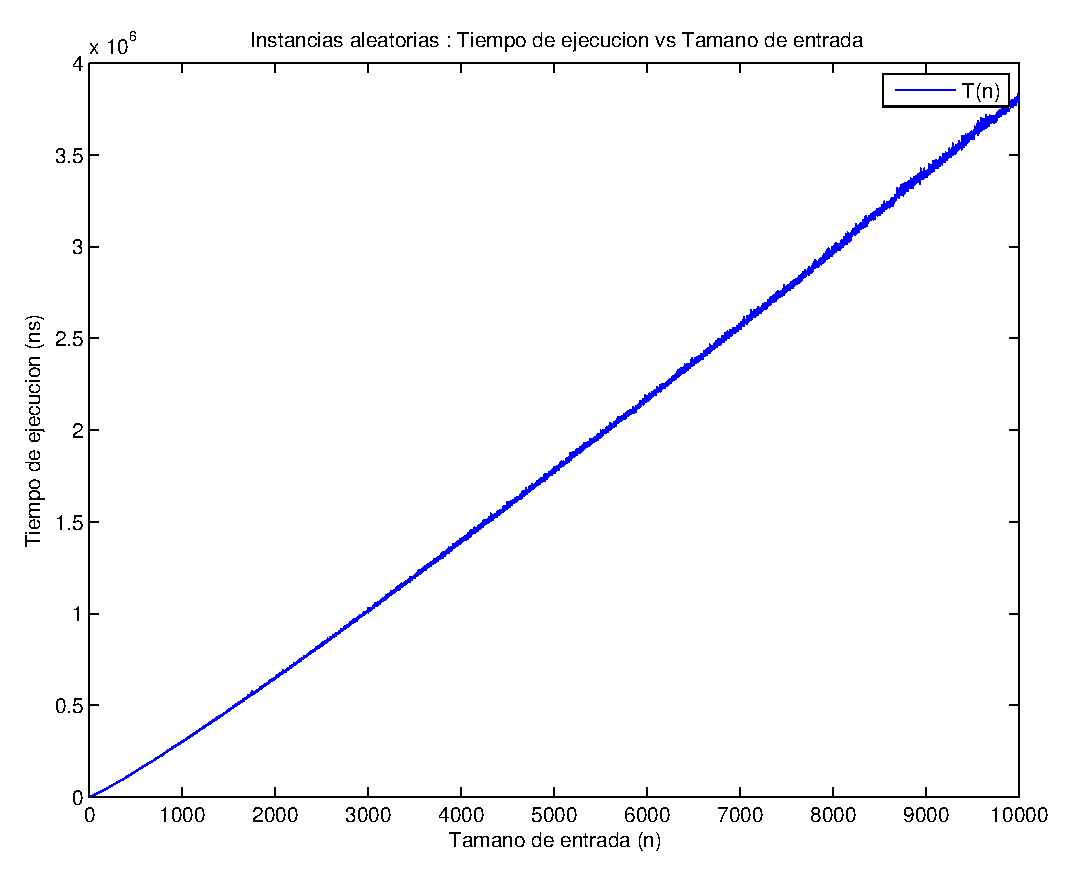
\includegraphics[width=0.5\linewidth]{problema2/graficos/problema2_aleatoria_10000.eps}
    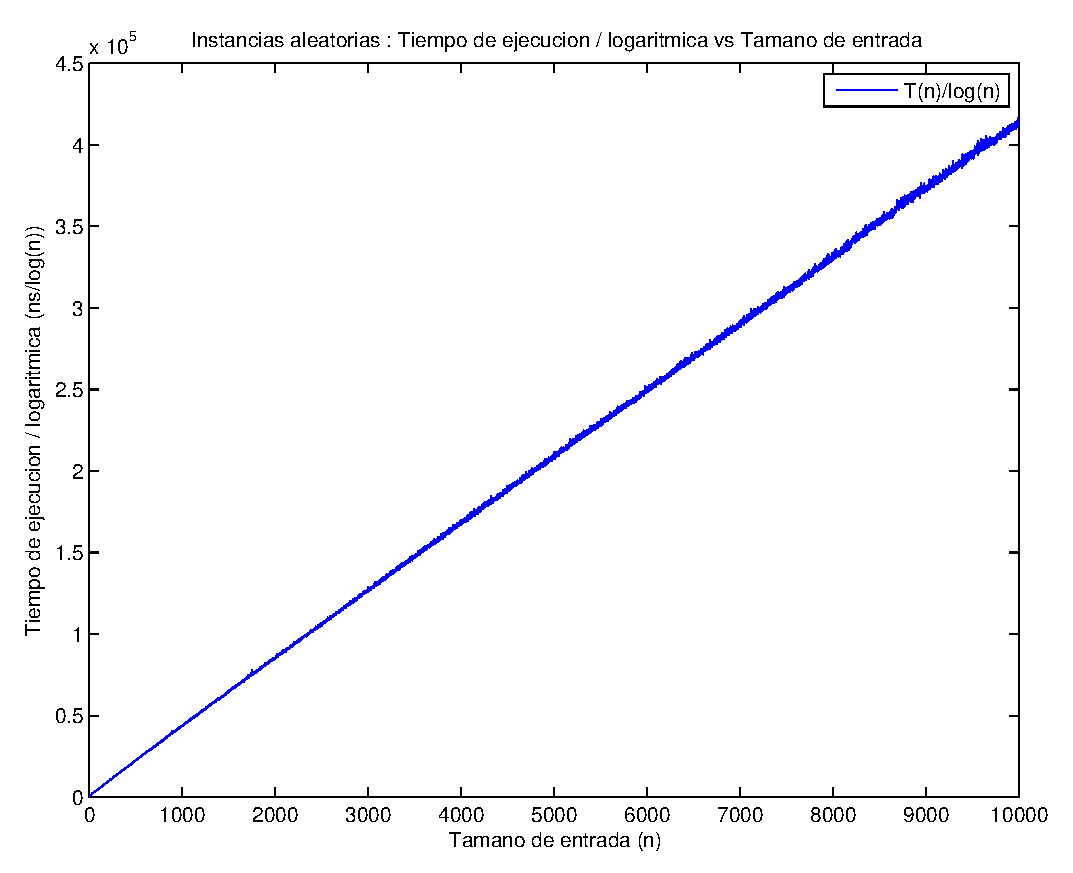
\includegraphics[width=0.5\linewidth]{problema2/graficos/problema2_aleatoria_10000_div_logn.eps}
\end{figure}
\emph{\hspace{2,5cm}Figura 1: Caso n = 10000 \hspace{2,5cm}Figura 2: Idem, pero dividido por $log(n)$}

Como se puede observar en la figura 2, una vez que dividimos por $log(n)$ a cada resultado obtenido por nuestras mediciones, éstos forman una recta. Es decir, $T(n)/log(n) \in O(n)$. Esto significa que la complejidad del algoritmo en su totalidad es de $O(n * log(n))$.
  
Según nuestro análisis, la complejidad temporal de la solución es dominada por la etapa de ordenamiento una vez más. Dado que el algoritmo utilizado para este fin es el mismo que el utilizado en el problema 1, de nuevo la experimentación subsiguiente se realizó sobre instancias donde la lista de entrada se encuentra ordenada, eliminando la etapa de ordenamiento. Esto permitió constatar si el resto del algoritmo incurre efectivamente en un costo a lo sumo lineal, y verificar la preponderancia del ordenamiento como parte de la solución.

En las figuras siguientes podemos observar que, sin contar la etapa de ordenamiento, efectivamente nuestro algoritmo es $O(n)$. Para lograr esto, utilizamos entradas en las cuales las joyas estén ordenadas según el coeficiente anteriormente mencionado, y por esto no haga falta realizar el sorting.

\begin{figure}[H]
    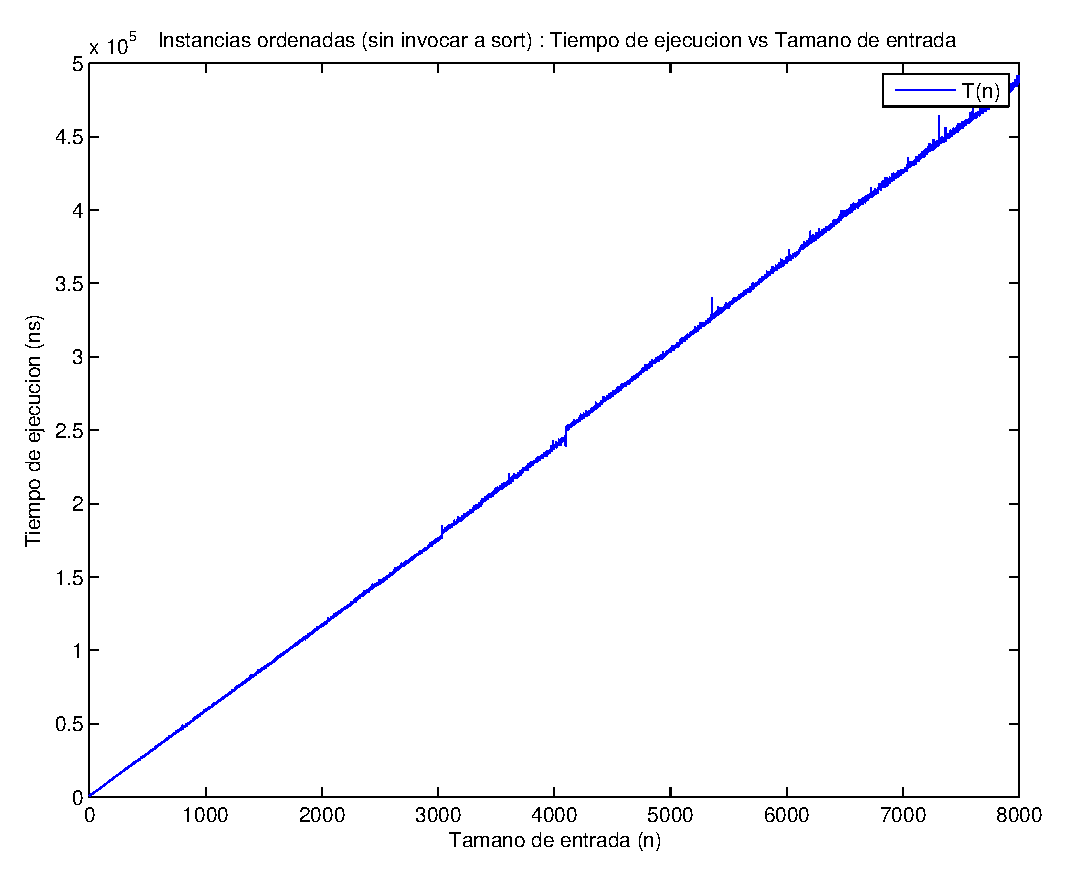
\includegraphics[width=0.5\linewidth]{problema2/graficos/problema2_ordenada_8000.eps}
    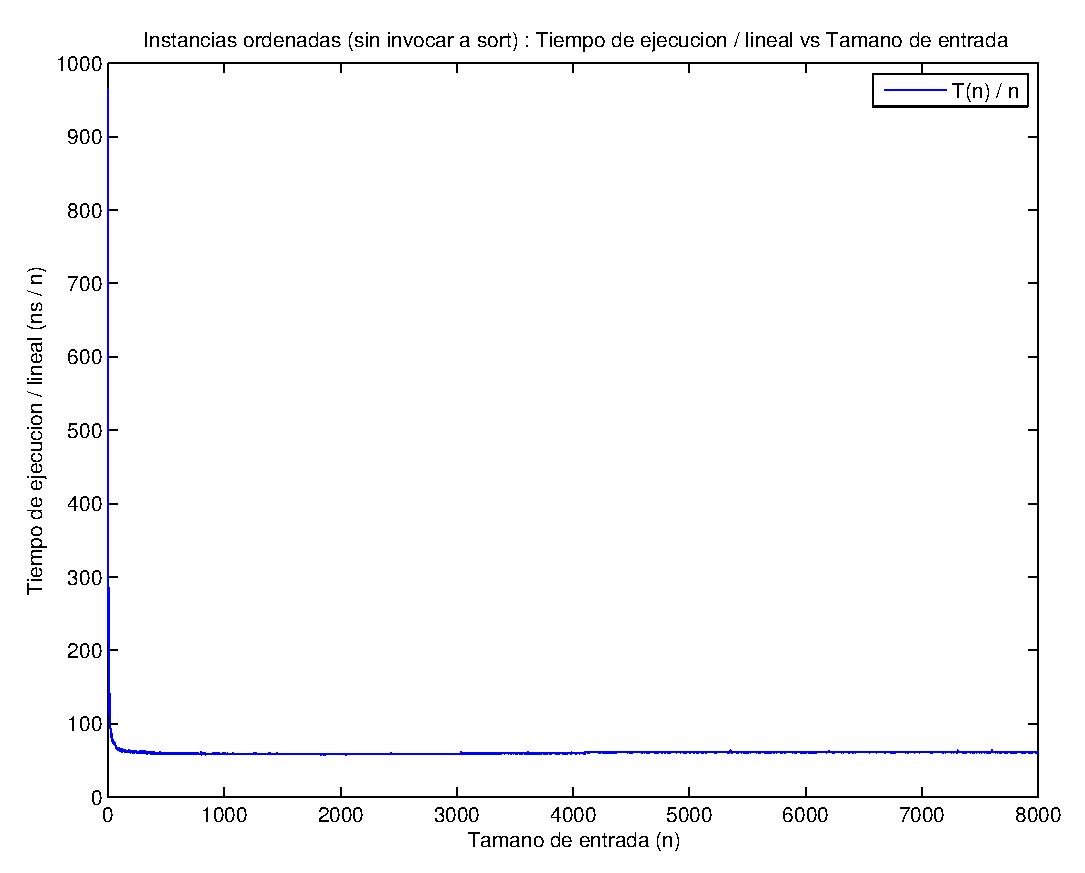
\includegraphics[width=0.5\linewidth]{problema2/graficos/problema2_ordenada_8000_div_n.eps}
\end{figure}
\emph{\hspace{2,5cm}Figura 3: Caso n = 8000 \hspace{3cm}Figura 4: Idem, pero dividido por $n$}

Como se puede observar en la figura 4, nuevamente al dividir por $n$ a cada resultado obtenido por nuestras mediciones, éstos se agrupan en una constante. Es decir, $T(n)/n \in O(1)$. Esto significa que la complejidad del algoritmo en su totalidad es de $O(n)$.

Cabe aclarar que en el caso de este problema, al remover la etapa de ordenamiento no existe ni mejor caso ni peor caso (O, mejor dicho, todos los casos son $\theta$(n)). Esto se debe a que este algoritmo recorre una vez el vector para guardar los datos, y una vez más para calcular las pérdidas. Siempre realiza esto, sin importar los datos.

En este problema tuvimos dificultades similares a las del ejercicio 1 en cuanto a determinar cuál es el peor y el mejor caso del algoritmo, ya que usamos un algoritmo de ordenamiento de las librerías de C++ y como éste usa en general el algoritmo de \emph{QuickSort}(en realidad usa \emph{IntroSort} ya explicado anteriormente), depende del azar el hecho de que ordenar un vector tarde más o menos comparaciones (siempre manteniéndose en el orden de complejidad temporal de $O(n * log n)$).

Pero además en este ejercicio que un caso sea peor o mejor depende exclusivamente de cuanto tarde el algoritmo en ordenar la entrada, ya que luego de esto sólo recorre el vector para calcular la pérdida total y devuelve dicho vector, esto siempre toma la misma cantidad de pasos, por lo tanto no nos es posible determinar \emph{a priori} si un caso va a resultar mejor o peor para este algoritmo.

%Por otro lado, como utilizamos el \emph{sort} de la \emph{stl}, no podemos asegurar si un caso en particular va a ser un ``mejor caso'', o un ``peor caso''. Esto se debe a que, como explicamos anteriormente, el sorting utiliza un \emph{IntroSort} que usa primordialmente un algoritmo similar a \emph{QuickSort}. Por esto al depender del azar, no se puede saber \emph{a priori} si un caso va a ser un ``mejor caso'', o un ``peor caso''.

%Por estas razones, para el ejercicio 2 no incluimos gráficos extra en los cuales hablamos de ``peor caso'' y ``mejor caso''.